% Options for packages loaded elsewhere
\PassOptionsToPackage{unicode}{hyperref}
\PassOptionsToPackage{hyphens}{url}
%
\documentclass[
]{article}
\usepackage{amsmath,amssymb}
\usepackage{lmodern}
\usepackage{iftex}
\ifPDFTeX
  \usepackage[T1]{fontenc}
  \usepackage[utf8]{inputenc}
  \usepackage{textcomp} % provide euro and other symbols
\else % if luatex or xetex
  \usepackage{unicode-math}
  \defaultfontfeatures{Scale=MatchLowercase}
  \defaultfontfeatures[\rmfamily]{Ligatures=TeX,Scale=1}
\fi
% Use upquote if available, for straight quotes in verbatim environments
\IfFileExists{upquote.sty}{\usepackage{upquote}}{}
\IfFileExists{microtype.sty}{% use microtype if available
  \usepackage[]{microtype}
  \UseMicrotypeSet[protrusion]{basicmath} % disable protrusion for tt fonts
}{}
\makeatletter
\@ifundefined{KOMAClassName}{% if non-KOMA class
  \IfFileExists{parskip.sty}{%
    \usepackage{parskip}
  }{% else
    \setlength{\parindent}{0pt}
    \setlength{\parskip}{6pt plus 2pt minus 1pt}}
}{% if KOMA class
  \KOMAoptions{parskip=half}}
\makeatother
\usepackage{xcolor}
\IfFileExists{xurl.sty}{\usepackage{xurl}}{} % add URL line breaks if available
\IfFileExists{bookmark.sty}{\usepackage{bookmark}}{\usepackage{hyperref}}
\hypersetup{
  hidelinks,
  pdfcreator={LaTeX via pandoc}}
\urlstyle{same} % disable monospaced font for URLs
\usepackage{color}
\usepackage{fancyvrb}
\newcommand{\VerbBar}{|}
\newcommand{\VERB}{\Verb[commandchars=\\\{\}]}
\DefineVerbatimEnvironment{Highlighting}{Verbatim}{commandchars=\\\{\}}
% Add ',fontsize=\small' for more characters per line
\newenvironment{Shaded}{}{}
\newcommand{\AlertTok}[1]{\textcolor[rgb]{1.00,0.00,0.00}{\textbf{#1}}}
\newcommand{\AnnotationTok}[1]{\textcolor[rgb]{0.38,0.63,0.69}{\textbf{\textit{#1}}}}
\newcommand{\AttributeTok}[1]{\textcolor[rgb]{0.49,0.56,0.16}{#1}}
\newcommand{\BaseNTok}[1]{\textcolor[rgb]{0.25,0.63,0.44}{#1}}
\newcommand{\BuiltInTok}[1]{#1}
\newcommand{\CharTok}[1]{\textcolor[rgb]{0.25,0.44,0.63}{#1}}
\newcommand{\CommentTok}[1]{\textcolor[rgb]{0.38,0.63,0.69}{\textit{#1}}}
\newcommand{\CommentVarTok}[1]{\textcolor[rgb]{0.38,0.63,0.69}{\textbf{\textit{#1}}}}
\newcommand{\ConstantTok}[1]{\textcolor[rgb]{0.53,0.00,0.00}{#1}}
\newcommand{\ControlFlowTok}[1]{\textcolor[rgb]{0.00,0.44,0.13}{\textbf{#1}}}
\newcommand{\DataTypeTok}[1]{\textcolor[rgb]{0.56,0.13,0.00}{#1}}
\newcommand{\DecValTok}[1]{\textcolor[rgb]{0.25,0.63,0.44}{#1}}
\newcommand{\DocumentationTok}[1]{\textcolor[rgb]{0.73,0.13,0.13}{\textit{#1}}}
\newcommand{\ErrorTok}[1]{\textcolor[rgb]{1.00,0.00,0.00}{\textbf{#1}}}
\newcommand{\ExtensionTok}[1]{#1}
\newcommand{\FloatTok}[1]{\textcolor[rgb]{0.25,0.63,0.44}{#1}}
\newcommand{\FunctionTok}[1]{\textcolor[rgb]{0.02,0.16,0.49}{#1}}
\newcommand{\ImportTok}[1]{#1}
\newcommand{\InformationTok}[1]{\textcolor[rgb]{0.38,0.63,0.69}{\textbf{\textit{#1}}}}
\newcommand{\KeywordTok}[1]{\textcolor[rgb]{0.00,0.44,0.13}{\textbf{#1}}}
\newcommand{\NormalTok}[1]{#1}
\newcommand{\OperatorTok}[1]{\textcolor[rgb]{0.40,0.40,0.40}{#1}}
\newcommand{\OtherTok}[1]{\textcolor[rgb]{0.00,0.44,0.13}{#1}}
\newcommand{\PreprocessorTok}[1]{\textcolor[rgb]{0.74,0.48,0.00}{#1}}
\newcommand{\RegionMarkerTok}[1]{#1}
\newcommand{\SpecialCharTok}[1]{\textcolor[rgb]{0.25,0.44,0.63}{#1}}
\newcommand{\SpecialStringTok}[1]{\textcolor[rgb]{0.73,0.40,0.53}{#1}}
\newcommand{\StringTok}[1]{\textcolor[rgb]{0.25,0.44,0.63}{#1}}
\newcommand{\VariableTok}[1]{\textcolor[rgb]{0.10,0.09,0.49}{#1}}
\newcommand{\VerbatimStringTok}[1]{\textcolor[rgb]{0.25,0.44,0.63}{#1}}
\newcommand{\WarningTok}[1]{\textcolor[rgb]{0.38,0.63,0.69}{\textbf{\textit{#1}}}}
\usepackage{graphicx}
\makeatletter
\def\maxwidth{\ifdim\Gin@nat@width>\linewidth\linewidth\else\Gin@nat@width\fi}
\def\maxheight{\ifdim\Gin@nat@height>\textheight\textheight\else\Gin@nat@height\fi}
\makeatother
% Scale images if necessary, so that they will not overflow the page
% margins by default, and it is still possible to overwrite the defaults
% using explicit options in \includegraphics[width, height, ...]{}
\setkeys{Gin}{width=\maxwidth,height=\maxheight,keepaspectratio}
% Set default figure placement to htbp
\makeatletter
\def\fps@figure{htbp}
\makeatother
\setlength{\emergencystretch}{3em} % prevent overfull lines
\providecommand{\tightlist}{%
  \setlength{\itemsep}{0pt}\setlength{\parskip}{0pt}}
\setcounter{secnumdepth}{-\maxdimen} % remove section numbering
\ifLuaTeX
  \usepackage{selnolig}  % disable illegal ligatures
\fi

\author{}
\date{}

\begin{document}

\hypertarget{kubernetes-ai-agent}{%
\section{Kubernetes AI Agent}\label{kubernetes-ai-agent}}

A large language model agent capable of monitoring a Kubernetes cluster.
This agent can be used to analyse metrics and logs to run diagnostics if
any issue is detected, identifying the root cause of the problem. The
agent will then provide a solution to the problem and document each step
in an incident report.

This project is the result of the Bachelor's final project by Alen
Bijelic during his final year at the School of Engineering and
Management, Haute Ecole d'Ingénierie et de Gestion du Canton de Vaud
(HEIG-VD). The project was supervised by Prof.~Marcel Graf.

\hypertarget{agent-workflow}{%
\subsection{Agent workflow}\label{agent-workflow}}

\begin{figure}
\centering
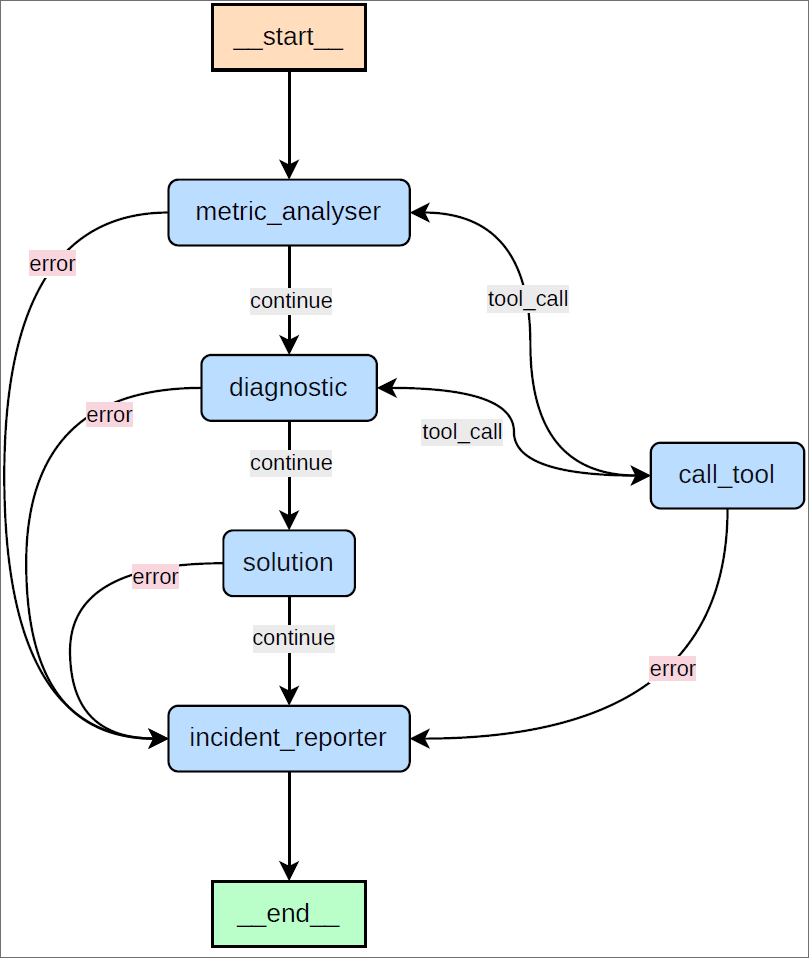
\includegraphics{img/realisation_langgraphworkflow.png}
\caption{Graph flow}
\end{figure}

\hypertarget{technology-stack}{%
\subsection{Technology Stack}\label{technology-stack}}

\begin{itemize}
\tightlist
\item
  \href{https://github.com/tiangolo/full-stack-fastapi-template}{\textbf{Full
  Stack FastAPI Template}} for the backend, frontend and DB.
\item
  \href{https://langchain-ai.github.io/langgraph/}{\textbf{LangGraph}}
  and \href{https://www.langchain.com/}{\textbf{LangChain}} for the AI
  agent.
\item
  \href{https://cloud.google.com/kubernetes-engine}{\textbf{Google
  Kubernetes Engine}} for the Kubernetes cluster.
\item
  \href{https://prometheus.io/}{\textbf{Prometheus}} for monitoring.
\end{itemize}

\hypertarget{how-to-use-it}{%
\subsection{How To Use It}\label{how-to-use-it}}

You can \textbf{just fork or clone} this repository and use it as is.

✨ It just works. ✨

\hypertarget{how-to-use-a-private-repository}{%
\subsubsection{How to Use a Private
Repository}\label{how-to-use-a-private-repository}}

If you want to have a private repository, GitHub won't allow you to
simply fork it as it doesn't allow changing the visibility of forks.

But you can do the following:

\begin{itemize}
\tightlist
\item
  Create a new GitHub repo, for example \texttt{my-full-stack}.
\item
  Clone this repository manually, set the name with the name of the
  project you want to use, for example \texttt{my-full-stack}:
\end{itemize}

\begin{Shaded}
\begin{Highlighting}[]
\FunctionTok{git}\NormalTok{ clone git@github.com:tiangolo/full{-}stack{-}fastapi{-}template.git my{-}full{-}stack}
\end{Highlighting}
\end{Shaded}

\begin{itemize}
\tightlist
\item
  Enter into the new directory:
\end{itemize}

\begin{Shaded}
\begin{Highlighting}[]
\BuiltInTok{cd}\NormalTok{ my{-}full{-}stack}
\end{Highlighting}
\end{Shaded}

\begin{itemize}
\tightlist
\item
  Set the new origin to your new repository, copy it from the GitHub
  interface, for example:
\end{itemize}

\begin{Shaded}
\begin{Highlighting}[]
\FunctionTok{git}\NormalTok{ remote set{-}url origin git@github.com:octocat/my{-}full{-}stack.git}
\end{Highlighting}
\end{Shaded}

\begin{itemize}
\tightlist
\item
  Add this repo as another ``remote'' to allow you to get updates later:
\end{itemize}

\begin{Shaded}
\begin{Highlighting}[]
\FunctionTok{git}\NormalTok{ remote add upstream git@github.com:tiangolo/full{-}stack{-}fastapi{-}template.git}
\end{Highlighting}
\end{Shaded}

\begin{itemize}
\tightlist
\item
  Push the code to your new repository:
\end{itemize}

\begin{Shaded}
\begin{Highlighting}[]
\FunctionTok{git}\NormalTok{ push }\AttributeTok{{-}u}\NormalTok{ origin master}
\end{Highlighting}
\end{Shaded}

\hypertarget{update-from-the-original-template}{%
\subsubsection{Update From the Original
Template}\label{update-from-the-original-template}}

After cloning the repository, and after doing changes, you might want to
get the latest changes from this original template.

\begin{itemize}
\tightlist
\item
  Make sure you added the original repository as a remote, you can check
  it with:
\end{itemize}

\begin{Shaded}
\begin{Highlighting}[]
\FunctionTok{git}\NormalTok{ remote }\AttributeTok{{-}v}

\ExtensionTok{origin}\NormalTok{    git@github.com:octocat/my{-}full{-}stack.git }\ErrorTok{(}\ExtensionTok{fetch}\KeywordTok{)}
\ExtensionTok{origin}\NormalTok{    git@github.com:octocat/my{-}full{-}stack.git }\ErrorTok{(}\ExtensionTok{push}\KeywordTok{)}
\ExtensionTok{upstream}\NormalTok{    git@github.com:tiangolo/full{-}stack{-}fastapi{-}template.git }\ErrorTok{(}\ExtensionTok{fetch}\KeywordTok{)}
\ExtensionTok{upstream}\NormalTok{    git@github.com:tiangolo/full{-}stack{-}fastapi{-}template.git }\ErrorTok{(}\ExtensionTok{push}\KeywordTok{)}
\end{Highlighting}
\end{Shaded}

\begin{itemize}
\tightlist
\item
  Pull the latest changes without merging:
\end{itemize}

\begin{Shaded}
\begin{Highlighting}[]
\FunctionTok{git}\NormalTok{ pull }\AttributeTok{{-}{-}no{-}commit}\NormalTok{ upstream master}
\end{Highlighting}
\end{Shaded}

This will download the latest changes from this template without
committing them, that way you can check everything is right before
committing.

\begin{itemize}
\item
  If there are conflicts, solve them in your editor.
\item
  Once you are done, commit the changes:
\end{itemize}

\begin{Shaded}
\begin{Highlighting}[]
\FunctionTok{git}\NormalTok{ merge }\AttributeTok{{-}{-}continue}
\end{Highlighting}
\end{Shaded}

\hypertarget{configure}{%
\subsubsection{Configure}\label{configure}}

You can then update configs in the \texttt{.env} files to customize your
configurations.

Before deploying it, make sure you change at least the values for:

\begin{itemize}
\tightlist
\item
  \texttt{SECRET\_KEY}
\item
  \texttt{FIRST\_SUPERUSER\_PASSWORD}
\item
  \texttt{POSTGRES\_PASSWORD}
\end{itemize}

You can (and should) pass these as environment variables from secrets.

Read the \href{./deployment.md}{deployment.md} docs for more details.

\hypertarget{generate-secret-keys}{%
\subsubsection{Generate Secret Keys}\label{generate-secret-keys}}

Some environment variables in the \texttt{.env} file have a default
value of \texttt{changethis}.

You have to change them with a secret key, to generate secret keys you
can run the following command:

\begin{Shaded}
\begin{Highlighting}[]
\ExtensionTok{python} \AttributeTok{{-}c} \StringTok{"import secrets; print(secrets.token\_urlsafe(32))"}
\end{Highlighting}
\end{Shaded}

Copy the content and use that as password / secret key. And run that
again to generate another secure key.

\hypertarget{how-to-use-it---alternative-with-copier}{%
\subsection{How To Use It - Alternative With
Copier}\label{how-to-use-it---alternative-with-copier}}

This repository also supports generating a new project using
\href{https://copier.readthedocs.io}{Copier}.

It will copy all the files, ask you configuration questions, and update
the \texttt{.env} files with your answers.

\hypertarget{install-copier}{%
\subsubsection{Install Copier}\label{install-copier}}

You can install Copier with:

\begin{Shaded}
\begin{Highlighting}[]
\ExtensionTok{pip}\NormalTok{ install copier}
\end{Highlighting}
\end{Shaded}

Or better, if you have \href{https://pipx.pypa.io/}{\texttt{pipx}}, you
can run it with:

\begin{Shaded}
\begin{Highlighting}[]
\ExtensionTok{pipx}\NormalTok{ install copier}
\end{Highlighting}
\end{Shaded}

\textbf{Note}: If you have \texttt{pipx}, installing copier is optional,
you could run it directly.

\hypertarget{generate-a-project-with-copier}{%
\subsubsection{Generate a Project With
Copier}\label{generate-a-project-with-copier}}

Decide a name for your new project's directory, you will use it below.
For example, \texttt{my-awesome-project}.

Go to the directory that will be the parent of your project, and run the
command with your project's name:

\begin{Shaded}
\begin{Highlighting}[]
\ExtensionTok{copier}\NormalTok{ copy https://github.com/tiangolo/full{-}stack{-}fastapi{-}template my{-}awesome{-}project }\AttributeTok{{-}{-}trust}
\end{Highlighting}
\end{Shaded}

If you have \texttt{pipx} and you didn't install \texttt{copier}, you
can run it directly:

\begin{Shaded}
\begin{Highlighting}[]
\ExtensionTok{pipx}\NormalTok{ run copier copy https://github.com/tiangolo/full{-}stack{-}fastapi{-}template my{-}awesome{-}project }\AttributeTok{{-}{-}trust}
\end{Highlighting}
\end{Shaded}

\textbf{Note} the \texttt{-\/-trust} option is necessary to be able to
execute a
\href{https://github.com/tiangolo/full-stack-fastapi-template/blob/master/.copier/update_dotenv.py}{post-creation
script} that updates your \texttt{.env} files.

\hypertarget{input-variables}{%
\subsubsection{Input Variables}\label{input-variables}}

Copier will ask you for some data, you might want to have at hand before
generating the project.

But don't worry, you can just update any of that in the \texttt{.env}
files afterwards.

The input variables, with their default values (some auto generated)
are:

\begin{itemize}
\tightlist
\item
  \texttt{project\_name}: (default: \texttt{"FastAPI\ Project"}) The
  name of the project, shown to API users (in .env).
\item
  \texttt{stack\_name}: (default: \texttt{"fastapi-project"}) The name
  of the stack used for Docker Compose labels and project name (no
  spaces, no periods) (in .env).
\item
  \texttt{secret\_key}: (default: \texttt{"changethis"}) The secret key
  for the project, used for security, stored in .env, you can generate
  one with the method above.
\item
  \texttt{first\_superuser}: (default: \texttt{"admin@example.com"}) The
  email of the first superuser (in .env).
\item
  \texttt{first\_superuser\_password}: (default: \texttt{"changethis"})
  The password of the first superuser (in .env).
\item
  \texttt{smtp\_host}: (default: ``\,``) The SMTP server host to send
  emails, you can set it later in .env.
\item
  \texttt{smtp\_user}: (default: ``\,``) The SMTP server user to send
  emails, you can set it later in .env.
\item
  \texttt{smtp\_password}: (default: ``\,``) The SMTP server password to
  send emails, you can set it later in .env.
\item
  \texttt{emails\_from\_email}: (default: \texttt{"info@example.com"})
  The email account to send emails from, you can set it later in .env.
\item
  \texttt{postgres\_password}: (default: \texttt{"changethis"}) The
  password for the PostgreSQL database, stored in .env, you can generate
  one with the method above.
\item
  \texttt{sentry\_dsn}: (default: ``\,``) The DSN for Sentry, if you are
  using it, you can set it later in .env.
\end{itemize}

\hypertarget{backend-development}{%
\subsection{Backend Development}\label{backend-development}}

Backend docs: \href{./backend/README.md}{backend/README.md}.

\hypertarget{frontend-development}{%
\subsection{Frontend Development}\label{frontend-development}}

Frontend docs: \href{./frontend/README.md}{frontend/README.md}.

\hypertarget{deployment}{%
\subsection{Deployment}\label{deployment}}

Deployment docs: \href{./deployment.md}{deployment.md}.

\hypertarget{development}{%
\subsection{Development}\label{development}}

General development docs: \href{./development.md}{development.md}.

This includes using Docker Compose, custom local domains, \texttt{.env}
configurations, etc.

\hypertarget{license}{%
\subsection{License}\label{license}}

The Kubernetes AI Agent is licensed under the terms of the MIT license.

\end{document}
